\documentclass{article}
\usepackage[utf8]{inputenc}
\usepackage[english]{babel}
\usepackage{geometry}
\usepackage[T1]{fontenc}
\usepackage{graphicx}
\graphicspath{ {../Figures/} }
\setlength\parindent{0pt}
\usepackage{hyperref}
\hypersetup{colorlinks=true,linkcolor=blue,filecolor=magenta,urlcolor=cyan,}
\urlstyle{same}
\usepackage{amsthm}
\usepackage{amsmath}
\theoremstyle{definition}
\usepackage{pgfplots}
\usepackage{caption}
\usepackage{subcaption}
\usepackage{makecell}
\usepackage[table]{colortbl}
\usepackage{enumitem}
\usepackage{siunitx}
\usepackage{amssymb}
\usepackage{tikz-cd}
\tikzset{>=latex}
\usepackage{tkz-euclide}
\usepackage{tikz,bm}
\usepackage{mwe,tikz}
\usetikzlibrary{arrows}
\pgfplotsset{compat=1.11}
\usepackage{moresize}
\usepackage{bohr}
\usetikzlibrary{patterns}
\usepackage{wrapfig}
\usepackage{mdframed}
\usepackage{dashrule}
\usepackage{tikzsymbols}
\usepackage{fontawesome}
\usepackage{multicol}
\usepackage{glossaries}
\usepackage{cancel}
% \usepackage{circuitikz}
\sisetup{group-separator = {,}}
\usepgfplotslibrary{fillbetween}
\usetikzlibrary{math}
\numberwithin{equation}{section}
\numberwithin{figure}{section}




\DeclareSIUnit{\nothing}{\relax}
\def\mymu{\SI{}{\micro\nothing} }

\newtheorem{example}{Example}[section]
\newtheorem{exercise}{}[section]
\newtheorem{regla}{Rule}


\newcommand{\Solution}{{\footnotesize \color{cyan} SOLUTION }}

\newcommand{\solutionEnd}{{\footnotesize \color{cyan} \hfill END OF SOLUTION }}

\newcommand{\cyanhrule}{{\color{cyan} \hrule }}

\def\redplus{\mathbin{\color{red} +}}
\def\redminus{\mathbin{\color{red} -}}
\def\redtimes{\mathbin{\color{red} \times}}


\def\openstax{https://openstax.org/books/physics/pages/1-introduction}
\def\openstaxfooter{\fancyfoot[C]{Access for free at \href{\openstax}{\openstax} \hfill \thepage}}


% The following needs to be added to each individual main.tex file so it doesn't interfere with exam headers:

%\usepackage{fancyhdr}
% \pagestyle{fancy}
% \renewcommand{\headrulewidth}{0pt}
% \renewcommand{\headruleskip}{0mm}
% \fancyhead{}
% \def\openstax{https://openstax.org/books/physics/pages/1-introduction}
% \def\openstaxfooter{\fancyfoot[C]{Access for free at \href{\openstax}{\openstax} \hfill \thepage}}

\newcommand\myboxa[2][]{\tikz[overlay]\node[fill=gray!20,inner sep=4pt, anchor=text, rectangle, rounded corners=1mm,#1] {#2};\phantom{#2}}

\newcommand{\hgraydashline}{{\color{lightgray} \hdashrule{0.99\textwidth}{1pt}{0.8mm}}}

\let\oldtexttt\texttt% Store \texttt
\renewcommand{\texttt}[2][black]{\textcolor{#1}{\ttfamily #2}}% 


\setlength{\columnsep}{1cm}
\setlength{\columnseprule}{1pt}
\def\columnseprulecolor{\color{cyan}}

\pgfdeclarehorizontalshading{visiblelight}{50bp}{
color(0.00000000000000bp)=(red);
color(8.33333333333333bp)=(orange);
color(16.66666666666670bp)=(yellow);
color(25.00000000000000bp)=(green);
color(33.33333333333330bp)=(cyan);
color(41.66666666666670bp)=(blue);
color(50.00000000000000bp)=(violet)
}

\def\myfillin{\rule{2cm}{0.15mm}}

\def\phet{\texttt[red]{PhET} }

\usepackage{circuitikz}

\usepackage{utfsym} %to get symbol of car
\def\mycar{\reflectbox{\huge\usym{1F697}} } %modiying symbol of car

\usepackage{mwe,tikz}

\usepackage{tikz}
\usetikzlibrary{positioning}
\usetikzlibrary{fadings,patterns}
\usepackage{tikzsymbols}

\newcommand\pgfmathsinandcos[3]{%
  \pgfmathsetmacro#1{sin(#3)}%
  \pgfmathsetmacro#2{cos(#3)}%
}

\newcommand\LatitudePlane[3][current plane]{%
  \pgfmathsinandcos\sinEl\cosEl{#2} % elevation
  \pgfmathsinandcos\sint\cost{#3} % latitude
  \pgfmathsetmacro\yshift{\cosEl*\sint}
  \tikzset{#1/.estyle={cm={\cost,0,0,\cost*\sinEl,(0,\yshift)}}} %
}

\newcommand\DrawLatitudeCircle[2][1]{
  \LatitudePlane{\angEl}{#2}
  \tikzset{current plane/.prefix style={scale=#1}}
  \pgfmathsetmacro\sinVis{sin(#2)/cos(#2)*sin(\angEl)/cos(\angEl)}
  % angle of "visibility"
  \pgfmathsetmacro\angVis{asin(min(1,max(\sinVis,-1)))}
  \draw[current plane,very thick,black] (\angVis:1) arc (\angVis:-\angVis-180:1);
  \draw[current plane,thin,dashed] (180-\angVis:1) arc (180-\angVis:\angVis:1);
}

\newcommand\DrawLatitudeCircleBack[2][1]{
  \LatitudePlane{\angEl}{#2}
  \tikzset{current plane/.prefix style={scale=#1}}
  \pgfmathsetmacro\sinVis{sin(#2)/cos(#2)*sin(\angEl)/cos(\angEl)}
  % angle of "visibility"
  \pgfmathsetmacro\angVis{asin(min(1,max(\sinVis,-1)))}
  %\draw[current plane,very thick,black] (\angVis:1) arc (\angVis:-\angVis-180:1);
  \draw[current plane,thin,dashed] (180-\angVis:1) arc (180-\angVis:\angVis:1);
}

\newcommand\DrawLatitudeCircleFront[2][1]{
  \LatitudePlane{\angEl}{#2}
  \tikzset{current plane/.prefix style={scale=#1}}
  \pgfmathsetmacro\sinVis{sin(#2)/cos(#2)*sin(\angEl)/cos(\angEl)}
  % angle of "visibility"
  \pgfmathsetmacro\angVis{asin(min(1,max(\sinVis,-1)))}
  \draw[current plane,very thick,black] (\angVis:1) arc (\angVis:-\angVis-180:1);
  %\draw[current plane,thin,dashed] (180-\angVis:1) arc (180-\angVis:\angVis:1);
}

\newcommand\DrawLatitudeCircleRedBack[2][1]{
  \LatitudePlane{\angEl}{#2}
  \tikzset{current plane/.prefix style={scale=#1}}
  \pgfmathsetmacro\sinVis{sin(#2)/cos(#2)*sin(\angEl)/cos(\angEl)}
  % angle of "visibility"
  \pgfmathsetmacro\angVis{asin(min(1,max(\sinVis,-1)))}
  \draw[current plane,thin,dashed,red] (180-\angVis:1) arc (180-\angVis:\angVis:1);
}

\newcommand\DrawLatitudeCircleRedFront[2][1]{
  \LatitudePlane{\angEl}{#2}
  \tikzset{current plane/.prefix style={scale=#1}}
  \pgfmathsetmacro\sinVis{sin(#2)/cos(#2)*sin(\angEl)/cos(\angEl)}
  % angle of "visibility"
  \pgfmathsetmacro\angVis{asin(min(1,max(\sinVis,-1)))}
  \draw[current plane,very thick,black,red] (\angVis:1) arc (\angVis:-\angVis-180:1);
}

\newcommand\FillLatitudeCircle[2][1]{
  \LatitudePlane{\angEl}{#2}
  \tikzset{current plane/.prefix style={scale=#1}}
  \pgfmathsetmacro\sinVis{sin(#2)/cos(#2)*sin(\angEl)/cos(\angEl)}
  % angle of "visibility"
  \pgfmathsetmacro\angVis{asin(min(1,max(\sinVis,-1)))}
  \fill[current plane,thin,lightgray] (\angVis:1) arc (\angVis:-\angVis-180:1);
  \fill[current plane,thin,dashed,lightgray] (180-\angVis:1) arc (180-\angVis:\angVis:1);
}

\tikzset{%
  >=latex,
  inner sep=0pt,%
  outer sep=2pt,%
  mark coordinate/.style={inner sep=0pt,outer sep=0pt,minimum size=3pt,
    fill=black,circle}%
}

\tikzfading[name=fade inside,
inner color=transparent!80,
outer color=transparent!30]





\newif\iflong %boolean
\longtrue %change to \longtrue (\longfalse) to show (hide) solutions.

    
\newcounter{mycounter}
\setcounter{mycounter}{1}

\begin{document}

\subsection{Observing the Sky (Unit 2)}

\begin{figure}[h!]
    \centering
\begin{tikzpicture}
\def\R{2.5} % sphere radius
\def\angEl{10} % elevation angle
\def\angBeta{25} % latitude of point P and Q


\pgfmathsetmacro\H{\R*cos(\angEl)} % distance to north pole
\node at (-0.2,0.7) {\small \textbf{E}};
\shade[ball color=white,opacity=0.5] (0,0) circle (\R);
\coordinate[mark coordinate] (O) at (0,0);

\begin{scope}[rotate=30]
    \DrawLatitudeCircleBack[\R]{0}
\end{scope}

\FillLatitudeCircle[\R]{0}
\DrawLatitudeCircle[\R]{0}

\draw[->] (0,0.15*\R) -- (0,1.01*\R) node[above] {Zenith};

\begin{scope}[rotate=30]
    \draw[thick] (0,\R) -- (0,\R*1.25) node[left=1pt,align=left] {North \\celestial\\ pole} (0,-\R) -- (0,-\R*1.25) node[right=1pt,align=left] {South \\celestial\\ pole};
    \draw[dashed,very thin] (0,\R) -- (0,0.2) (0,-0.22*\R) -- (0,-\R);
    \DrawLatitudeCircleFront[\R]{0}
\end{scope}

\draw (-\R*0.7,-\R*0.52) --++ (-\R*0.2,-\R*0.3) node[below left,align=left] {Celestial\\ equator};
\node[left] at (-\R,0) {\textbf{N}};
\node[right] at (\R,0) {\textbf{S}};
\draw (2,0.25) -- ++(1,0.7) node[right] {Horizon};

\node at (0,0.1) {\Strichmaxerl[1.8]};
\node at (1.3*\R,0.9*\R) {\large \textbf{Celestial Sphere}};
\node at (0.1,-\R*0.3) {\textbf{W}};
\end{tikzpicture}
\caption*{\textbf{Figure 2.3 Circles on the Celestial Sphere.}}
\end{figure}

\begin{figure}[h!]
    \centering
\begin{tikzpicture}
\def\R{2.5} % sphere radius
\def\angEl{10} % elevation angle
\def\angBeta{25} % latitude of point P and Q


\pgfmathsetmacro\H{\R*cos(\angEl)} % distance to north pole
\node at (-0.2,0.7) {\small \textbf{E}};
\shade[ball color=white,opacity=0.5] (0,0) circle (\R);
\coordinate[mark coordinate] (O) at (0,0);

\begin{scope}[rotate=30]
    \DrawLatitudeCircleBack[\R]{0}
\end{scope}

\FillLatitudeCircle[\R]{0}
\DrawLatitudeCircle[\R]{0}

\draw[->] (0,0.15*\R) -- (0,1.01*\R) node[above] {\framebox{\textbf{A}}};

\begin{scope}[rotate=30]
    \draw[thick] (0,\R) -- (0,\R*1.25) node[left=1pt,align=left] {\framebox{\textbf{B}}} (0,-\R) -- (0,-\R*1.25) node[right=1pt,align=left] {\framebox{\textbf{C}}};
    \draw[dashed,very thin] (0,\R) -- (0,0.2) (0,-0.22*\R) -- (0,-\R);
    \DrawLatitudeCircleFront[\R]{0}
\end{scope}

\draw (-\R*0.7,-\R*0.52) --++ (-\R*0.2,-\R*0.3) node[below left,align=left] {\framebox{\textbf{D}}};
\node[left] at (-\R,0) {\textbf{N}};
\node[right] at (\R,0) {\textbf{S}};
\draw (2,0.25) -- ++(1,0.7) node[right] {\framebox{\textbf{E}}};

\node at (0,0.1) {\Strichmaxerl[1.8]};
\node at (0.8*\R,0.9*\R) {\framebox{\textbf{F}}};
\node at (0.1,-\R*0.3) {\textbf{W}};
\end{tikzpicture}
\caption*{\textbf{Figure 2.3 Circles on the Celestial Sphere.}}
\end{figure}

%%%%

\begin{figure}[h!]
\centering
\begin{tikzpicture}

\def\R{3} % sphere radius
\def\angEl{23} % elevation angle
\def\angTilt{30} %tilt angle increased from 23.5 for emphasis

\draw (0,0) -- (0,\R*1.25);

\draw[very thick,fill=yellow] (0.3,1.15) circle (3pt) node[above right] {\textbf{September}};

\begin{scope}[rotate=-\angTilt]
    \draw (0,1.25*\R) -- (0,0);
\end{scope}
\shade[ball color=white, opacity=0.5] (0,0) circle (\R);
\coordinate[mark coordinate] (O) at (0,0);

\begin{scope}[rotate=-\angTilt]
    \DrawLatitudeCircleBack[\R]{0}
\end{scope}

\begin{scope}[rotate=-\angTilt]
        \DrawLatitudeCircleFront[\R]{0}
        \draw[blue,thick]  (0,0) -- (0,1) (0,0) -- (0,-1); %(0,\R*1.25) -- (0,\R)
        \draw[very thick,blue,fill=white] (0,0) circle (19pt) node {\rotatebox{-\angTilt}{\textbf{Earth}}};
        \node at (0.25,0.9) {\textbf{N}};
        \node at (-0.2,-0.9) {\textbf{S}};
\end{scope}

\DrawLatitudeCircle[\R]{0}
\draw (-2,-0.9) --++ (-1.3,-0.6) node[below] {Ecliptic};

\draw[very thick,fill=yellow] (-\R,0) circle (4pt) node[left=7pt] {\textbf{December}};
\draw[very thick,fill=yellow] (\R,0) circle (4pt) node[right=6pt] {\textbf{June}};
\draw[very thick,fill=yellow] (-0.3,-1.15) circle (4pt) node[below=8pt] {\textbf{March}};

\draw[very thick,<->] (0,2.2) arc (90:55:1.85);
\node at (0.75,2.5) {\SI{23.5}{\degree}};

\draw (1.7,-1.8) -- ++(1,-0.4) node[right] {Celestial Equator};

\draw[very thick,<->] (1.7,-1) arc (-10:-45:1.4);
\node at (2.1,-1.45) {\small {\SI{23.5}{\degree}}};

\node at (-2.8,2.8) {Celestial Sphere};

\end{tikzpicture}
\caption*{\textbf{Figure 2.7 The Celestial Tilt}.}
\end{figure}

%%%%%%%%%%%%%%%%%%%%%%%%%%%%%%%%%%%%%%%%%%%%%%%%%%%%%%%%%%%%%%%%%%%%%%%%%%%%%%%%%

\begin{figure}[h!]
    \centering
\begin{tikzpicture}
\def\R{3} % sphere radius
\def\angEl{23} % elevation angle
\def\angTilt{30} %tilt angle increased from 23.5 for emphasis

\pgfmathsetmacro\H{\R*cos(\angEl)} % distance to north pole
\draw (0,0) -- (0,\H*1.25);
\draw[very thick,fill=yellow] (0.3,1.15) circle (3pt);%node[above right=-8pt] {\textbf{September}};

\begin{scope}[rotate=-\angTilt]
    \draw[very thin] (0,\H) -- (0,0);
\end{scope}
\shade[ball color=white,opacity=0.5] (0,0) circle (\R);
\coordinate[mark coordinate] (O) at (0,0);

\begin{scope}[rotate=-\angTilt]
    \DrawLatitudeCircleBack[\R]{0}
\end{scope}

\begin{scope}[rotate=-\angTilt]
        \DrawLatitudeCircleFront[\R]{0}
        \draw[thick] (0,\H*1.25) -- (0,\H) (0,0) -- (0,-1);
        \draw[very thick,blue,fill=white] (0,0) circle (19pt) node {\rotatebox{-\angTilt}{\textbf{Earth}}};
        \node at (0.2,0.9) {\textbf{N}};
        \node at (-0.2,-0.9) {\textbf{S}};
\end{scope}

\DrawLatitudeCircle[\R]{0}
\draw (-2,-0.9) --++ (-1.3,-0.6) node[left] {\framebox{\textbf{D}}};

\draw[very thick,fill=yellow] (-\R,0) circle (4pt);

\draw[very thick, fill=yellow] (\R,0) circle (4pt);
\draw (\R,0) -- ++ (1,1) node[right] {\framebox{\textbf{E}}};

\draw[very thick,fill=yellow] (-0.3,-1.15) circle (4pt);

\draw[very thick,<->] (0,2.3) arc (90:55:1.85);
\node at (0.7,2.6) {\framebox{\textbf{B}}};

\draw[thick] (1.7,-1.8) -- ++(1,-0.4) node[right] {\framebox{\textbf{A}}};

\node at (-1.05,0.2) {\framebox{\textbf{C}}};
\end{tikzpicture}
\end{figure}

%%%%%

Astronomy \hfill Worksheet \themycounter \hfill Chapter 2
\vspace{1em}

\begin{center} 
\fbox{\fbox{\parbox{5.5in}{\centering \textbf{Directions}: }}}
\end{center}

\textbf{Zenith}
\vspace{-1em}

\begin{enumerate}
\setlength\itemsep{0pt}
    \item Open \textit{Stellarium}.
    \item Click \texttt[red]{Location window [F6]} and set location to \textit{Cypress, Texas}. Close the window.
    \item Click \texttt[red]{Date/time window [F5]} and set the date/time to today at midnight (or any time that's dark). Close the window.
    \item Click \texttt[red]{Sky and viewing options window [F4]} and click the \texttt[red]{Markings} tab.
    \item Check \texttt[red]{Zenith and Nadir}. Close the window. \item Search the celestial sphere for the zenith. Where is it? Record your observations.
    \item Change the location to \textit{Lima, Per\'{u}}. Search for the zenith again, recording your observations.
    \item Based on your observations, create your own definition of \textbf{zenith}.
    \item What is the textbook definition of zenith?
\end{enumerate}

\textbf{Horizon}
\vspace{-1em}

\begin{enumerate}
\setlength\itemsep{0pt}
    \item Open \textit{Stellarium}.
    \item Click \texttt[red]{Location window [F6]} and set location to \textit{Cypress, Texas}. Close the window.
    \item Click \texttt[red]{Date/time window [F5]} and set the date/time to today at noon (or any time during the day). Close the window.
    \item Click \texttt[red]{Sky and viewing options window [F4]} and click the \texttt[red]{Markings} tab. 
    \item Check the first \texttt[red]{Horizon} box.
    \item Click the \texttt[red]{Landscape} tab. Under \texttt[red]{Options}, un-check the \texttt[red]{Show ground} box. 
    \item Re-check and un-check the \texttt[red]{Show ground} box as you explore the surroundings. Record your observations. 
    \item Based on your observations, create your own definition of \textbf{horizon}.
    \item What is the textbook definition of \textbf{horizon}?
\end{enumerate}

\clearpage

\stepcounter{mycounter}
Astronomy \hfill Worksheet \themycounter \hfill Chapter 2
\vspace{1em}

\textbf{Celestial Poles}
\vspace{-1em}

\begin{enumerate}
\setlength\itemsep{0pt}
    \item Open \textit{Stellarium}.
    \item Click \texttt[red]{Location window [F6]} and set location to \textit{Cypress, Texas}. Close the window.
    \item Click \texttt[red]{Sky and viewing options window [F4]}. Under the \texttt[red]{Sky} tab, in the \texttt[red]{Sky} section, un-check the \texttt[red]{Atmosphere visualization} box. This shows what the sky would look like without an atmosphere. 
    \item Click \texttt[red]{Markings} tab. Check the \texttt[red]{Celestial Poles~(J2000)} box, and close the window.
    \item Find the north celestial pole (NCP) in the sky. Ensure that it and the horizon is visible.
    \item Press the keyboard \framebox{\texttt[red]{L}} key repeatedly as needed to advance time (or \framebox{\texttt[red]{K}} to pause or \framebox{\texttt[red]{J}} to rewind). What do you notice about the north celestial pole as time progresses? \\Record your observations.
    \item Based on your observations, create your own definition of \textbf{celestial pole}.
    \item What is the textbook definition of \textbf{celestial pole}?
    \item The so-called ``North Star'' is a bright star that is conveniently located near the NCP. Pre-modern navigators used  the North Star to locate the northward direction and, therefore, the 3 other cardinal directions. According to \textit{Stellarium}, what is the actual name of the North Star? \\(\textit{Tip}: Try zooming in near the NCP.)
\end{enumerate}

\textbf{Celestial Equator}
\vspace{-1em}

\begin{enumerate}
\setlength\itemsep{0pt}
    \item Open \textit{Stellarium}.
    \item Click \texttt[red]{Location window [F6]} and set location to \textit{Cypress, Texas}. Close the window.
    \item Click \texttt[red]{Sky and viewing options window [F4]}. Click the \texttt[red]{Markings} tab. Check the \texttt[red]{Celestial Poles~(J2000)} box and the first \texttt[red]{Equator~(J2000)} box. This shows the celestial equator. Set the \texttt{Thickness} of lines to 5. Close the window.
    \item Center the view towards the East, with the NCP and celestial equator in view. 
    \item Press the keyboard \framebox{\texttt[red]{L}} key 3 or 4 times to advance time (or \framebox{\texttt[red]{K}} to pause or \framebox{\texttt[red]{J}} to rewind). What do you notice about the celestial equator as time progresses? \\Record your observations.
    \item Based on your observation, create a definition for \textbf{celestial equator}.
    \item What is the textbook definition of \textbf{celestial equator}?
\end{enumerate}



\clearpage

\stepcounter{mycounter}
Astronomy \hfill Worksheet \themycounter \hfill Chapter 2
\vspace{1em}

\begin{enumerate}
\setlength\parskip{0pt}
    \item Open \textit{Stellarium}.
    \item Click \texttt[red]{Sky and viewing options window [F4]} and click the \texttt[red]{Markings} tab.
    \item Check \texttt[red]{Equator (J2000)} and set \texttt[red]{Thickness} of lines to 5. This displays the celestial equator in blue. Close the window.
    \item \label{lab:Stellarium_SetLocation} Open \texttt[red]{Location window [F6]} and set location to \textit{Longyearbyen}, one of the northern most towns in the world. Record the latitude of this location. 
    \item \label{lab:Stellarium_CelestialEquator} Describe the location of the \textbf{celestial equator} on the celestial sphere relative to the horizon and to the zenith using the sentence below: \textit{The celestial equator is \rule{2cm}{0.15mm} the horizon and it's \rule{2cm}{0.15mm} the zenith.}
    \item Repeat steps (\ref{lab:Stellarium_SetLocation}) and (\ref{lab:Stellarium_CelestialEquator}) using the equatorial city \textit{Nairobi}, southern city \textit{Ushuaia}, and 3 additional cities of your choice. 
\end{enumerate}

\begin{center}
    \begin{tabular}{|p{2.5cm}|p{2cm}|p{10cm}|}
        \hline
        \textbf{City} & \textbf{Latitude} & \textbf{Description of Celestial Equator} \\
        \hline
        Longyearbyen & & \\[3em]
        \hline
        Nairobi & & \\[3em]
        \hline
        Ushuaia & & \\[3em]
        \hline
        & & \\[3em]
        \hline
        & & \\[3em]
        \hline
        & & \\[3em]
        \hline
    \end{tabular}
\end{center}

\clearpage

\stepcounter{mycounter}
Astronomy \hfill Worksheet \themycounter \hfill Chapter 2
\vspace{1em}

\begin{center} 
\fbox{\fbox{\parbox{5.5in}{\textbf{Directions}: Using words from the Word Bank, fill in the blanks in the spaces provided on the figure.}}}
\end{center}

\begin{minipage}{0.3\textwidth}
\centering
\begin{tabular}{|l|}
    \hline
    \textbf{Word Bank}\\
    \hline
    North celestial pole\\
    South celestial pole\\
    Celestial equator\\
    Horizon\\
    Celestial Sphere\\
    Zenith\\
    \Strichmaxerl[1.8]\\
    \hline
\end{tabular}
\end{minipage}%
\hspace{1cm}
\begin{minipage}{0.49\textwidth}
\centering
\begin{tikzpicture}[scale=1,every node/.style={minimum size=1cm}]
\def\R{2.5} % sphere radius
\def\angEl{10} % elevation angle
\def\angBeta{25} % latitude of point P and Q

\node at (0.1,-\R*0.3) {\small \textbf{W}};
\pgfmathsetmacro\H{\R*cos(\angEl)} % distance to north pole
\node[left] at (0.35,0.7) {\small \textbf{E}};
\shade[ball color=white,opacity=0.5] (0,0) circle (\R);
\coordinate[mark coordinate] (O) at (0,0);


\begin{scope}[rotate=30]
    \DrawLatitudeCircleBack[\R]{0}
    \draw (0,\H*0.8) --++ (0,\H*0.2) node[above left=5pt,align=left]{\rule{1.5cm}{0.15mm}}; %NCP
    \draw (0,-\H*0.8) --++ (0,-\H*0.2) node[below right=18pt,align=left]{\rule{1.5cm}{0.15mm}}; %SCP
\end{scope}


\FillLatitudeCircle[\R]{0}
\DrawLatitudeCircle[\R]{0}

\draw[->] (0,0.15*\R) -- (0,\R) node[above=-8pt] {\rule{1.5cm}{0.15mm}}; %zenith

\begin{scope}[rotate=30]
    \draw[very thick] (0,\H*1.25) -- (0,\H) (0,-\H) -- (0,-\H*1.25);
    \draw[dashed,very thin] (0,\H) -- (0,0) (0,-0.3*\H) -- (0,-\H);
    \DrawLatitudeCircleFront[\R]{0}
\end{scope}

\draw (-\H*0.7,-\H*0.52) --++ (-\H*0.2,-\H*0.3) node[below=-6pt,align=left] {\rule{1.5cm}{0.15mm}}; %celestial equator
\node[left] at (-\R*0.9,0) {\textbf{N}};
\node[right] at (\R*0.9,0) {\textbf{S}};
\draw (2,0.25) -- ++(1,0.7) node[right] {\rule{1.5cm}{0.15mm}}; %horizon

\node at (1.3*\R,0.9*\R) {\rule{1.5cm}{0.15mm}}; %celestial sphere
\end{tikzpicture}
\end{minipage}

\vspace{2cm}

\begin{minipage}{0.3\textwidth}
\centering
\begin{tabular}{|l|}
    \hline
    \textbf{Word Bank}\\
    \hline
    Celestial sphere\\
    Celestial equator\\
    Ecliptic\\
    Earth\\
    December\\
    March\\
    June\\
    September\\
    \SI{23.5}{\degree}\\
    North celestial pole\\
    South celestial pole\\
    \hline
\end{tabular}
\end{minipage}%
\hspace{1cm}
\begin{minipage}{0.49\textwidth}
\centering
\begin{tikzpicture}[scale=1,every node/.style={minimum size=1cm}]

\def\R{3} % sphere radius
\def\angEl{23} % elevation angle
\def\angTilt{30} % latitude of point P and Q

\pgfmathsetmacro\H{\R*cos(\angEl)} % distance to north pole
\draw (0,0) -- (0,\H*1.25);
\fill[yellow] (0.3,1.15) circle (3pt);
\draw[very thick] (0.3,1.15) circle (3pt) node[above right=-8pt] {\rule{1cm}{0.15mm}}; %September

\begin{scope}[rotate=-\angTilt]
    \draw[very thin] (0,\H) -- (0,0);
\end{scope}
\shade[ball color=white,opacity=0.5] (0,0) circle (\R);
\coordinate[mark coordinate] (O) at (0,0);

\begin{scope}[rotate=-\angTilt]
    \DrawLatitudeCircleBack[\R]{0}
\end{scope}

\begin{scope}[rotate=-\angTilt]
        \DrawLatitudeCircleFront[\R]{0}
        \draw[thick] (0,\H*1.25) -- (0,\H) (0,0) -- (0,-0.8);
        \node at (0,0) {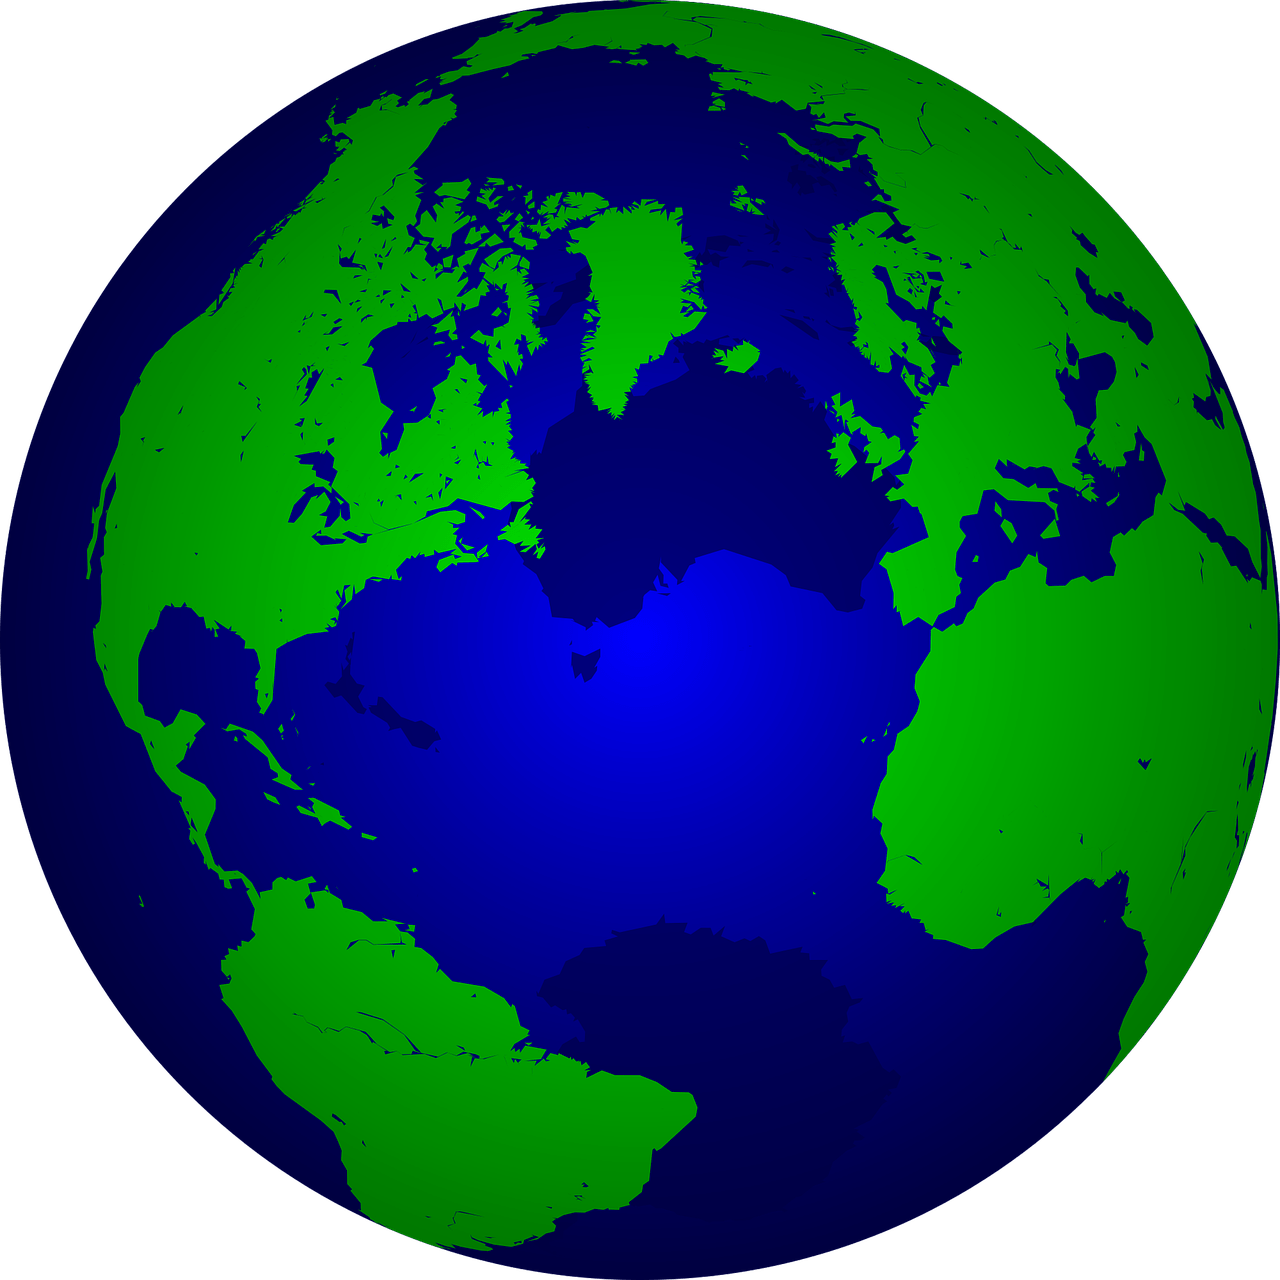
\includegraphics[width=1cm]{Figures/Earth.png}};
        \node at (0.3,0.8) {\textbf{N}};
        \node at (-0.3,-0.8) {\textbf{S}};
\end{scope}

\DrawLatitudeCircle[\R]{0}
\draw (-2,-0.9) --++ (-1.3,-0.6) node[below=-8pt] {\rule{1cm}{0.15mm}}; %Ecliptic

\fill[yellow] (-\R,0) circle (4pt); 
\draw[very thick] (-\R,0) circle (4pt) node[left=7pt] {\textbf{\rule{1cm}{0.15mm}}}; %December

\fill[yellow] (\R,0) circle (4pt);
\draw[very thick] (\R,0) circle (4pt) node[right=6pt] {\textbf{\rule{1cm}{0.15mm}}}; %June

\fill[yellow] (-0.3,-1.15) circle (4pt); 
\draw[very thick] (-0.3,-1.15) circle (4pt) node[below] {\textbf{\rule{1cm}{0.15mm}}}; %March

\draw[very thick,<->] (0,2.3) arc (90:55:1.85);
\node at (0.7,2.6) {\rule{1cm}{0.15mm}}; %23.5 degrees

\draw (1.7,-1.8) -- ++(1,-0.4) node[right] {\rule{1cm}{0.15mm}}; %Celestial equator

\draw[very thick,<->] (1.7,-1) arc (-10:-45:1.4);

\node at (-2.7,2.7) {\rule{1cm}{0.15mm}}; %Celestial Sphere
\end{tikzpicture}
\end{minipage}

\clearpage
\iflong
\begin{center}
    {\color{red} \textbf{SOLUTION}}
\end{center}

\begin{figure}[h!]
    \centering
\begin{tikzpicture}
\def\R{2.5} % sphere radius
\def\angEl{10} % elevation angle
\def\angBeta{25} % latitude of point P and Q


\pgfmathsetmacro\H{\R*cos(\angEl)} % distance to north pole
\node at (-0.2,0.7) {\small \textbf{E}};
\shade[ball color=white,opacity=0.5] (0,0) circle (\R);
\coordinate[mark coordinate] (O) at (0,0);

\begin{scope}[rotate=30]
    \DrawLatitudeCircleBack[\R]{0}
\end{scope}

\FillLatitudeCircle[\R]{0}
\DrawLatitudeCircle[\R]{0}

\draw[->] (0,0.15*\R) -- (0,1.01*\R) node[above] {Zenith};

\begin{scope}[rotate=30]
    \draw[thick] (0,\R) -- (0,\R*1.25) node[left=1pt,align=left] {North \\celestial\\ pole} (0,-\R) -- (0,-\R*1.25) node[right=1pt,align=left] {South \\celestial\\ pole};
    \draw[dashed,very thin] (0,\R) -- (0,0.2) (0,-0.22*\R) -- (0,-\R);
    \DrawLatitudeCircleFront[\R]{0}
\end{scope}

\draw (-\R*0.7,-\R*0.52) --++ (-\R*0.2,-\R*0.3) node[below left,align=left] {Celestial\\ equator};
\node[left] at (-\R,0) {\textbf{N}};
\node[right] at (\R,0) {\textbf{S}};
\draw (2,0.25) -- ++(1,0.7) node[right] {Horizon};

\node at (0,0.1) {\Strichmaxerl[1.8]};
\node at (1.3*\R,0.9*\R) {\large \textbf{Celestial Sphere}};
\node at (0.1,-\R*0.3) {\textbf{W}};
\end{tikzpicture}
\caption*{\textbf{Figure 2.3 Circles on the Celestial Sphere.}}
\end{figure}

\begin{figure}[h!]
\centering
\begin{tikzpicture}[scale=1,every node/.style={minimum size=1cm}]

\def\R{3} % sphere radius
\def\angEl{23} % elevation angle
\def\angTilt{30} % latitude of point P and Q

\pgfmathsetmacro\H{\R*cos(\angEl)} % distance to north pole
\draw (0,0) -- (0,\H*1.25);
\fill[yellow] (0.3,1.15) circle (3pt);
\draw[very thick] (0.3,1.15) circle (3pt) node[above right=-8pt] {\textbf{September}};

\begin{scope}[rotate=-\angTilt]
    \draw[very thin] (0,\H) -- (0,0);
\end{scope}
\shade[ball color=white,opacity=0.5] (0,0) circle (\R);
\coordinate[mark coordinate] (O) at (0,0);

\begin{scope}[rotate=-\angTilt]
    \DrawLatitudeCircleBack[\R]{0}
\end{scope}

\begin{scope}[rotate=-\angTilt]
        \DrawLatitudeCircleFront[\R]{0}
        \draw[thick] (0,\H*1.25) -- (0,\H) (0,0) -- (0,-0.8);
        \node at (0,0) {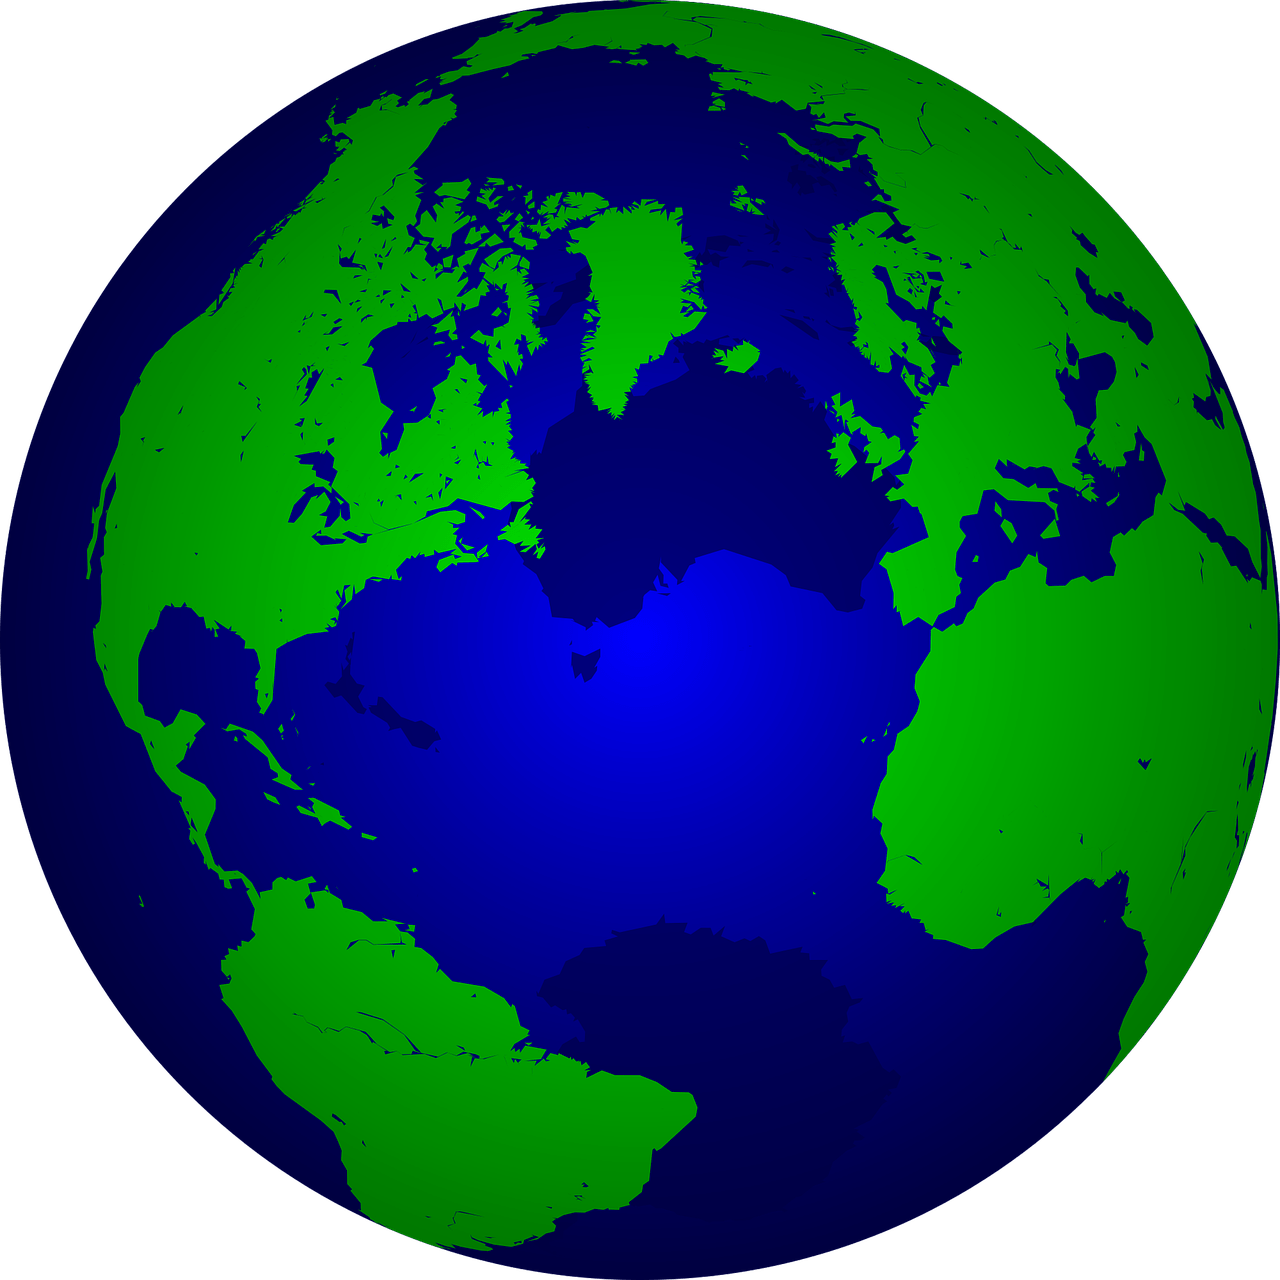
\includegraphics[width=1cm]{Figures/Earth.png}};
        \node at (0.3,0.8) {\textbf{N}};
        \node at (-0.3,-0.8) {\textbf{S}};
\end{scope}

\DrawLatitudeCircle[\R]{0}
\draw (-2,-0.9) --++ (-1.3,-0.6) node[below=-8pt] {Ecliptic};

\fill[yellow] (-\R,0) circle (4pt); 
\draw[very thick] (-\R,0) circle (4pt) node[left=7pt] {\textbf{December}};

\fill[yellow] (\R,0) circle (4pt);
\draw[very thick] (\R,0) circle (4pt) node[right=6pt] {\textbf{June}};

\fill[yellow] (-0.3,-1.15) circle (4pt); 
\draw[very thick] (-0.3,-1.15) circle (4pt) node[below] {\textbf{March}};

\draw[very thick,<->] (0,2.3) arc (90:55:1.85);
\node at (0.7,2.6) {\SI{23.5}{\degree}};

\draw (1.7,-1.8) -- ++(1,-0.4) node[right] {Celestial Equator};

\draw[very thick,<->] (1.7,-1) arc (-10:-45:1.4);
\node at (2.1,-1.45) {\small {\SI{23.5}{\degree}}};

\node at (-3,3) {Celestial Sphere};

\end{tikzpicture}
\end{figure}

\else \fi

\subsection{Earth, Moon, and Sky (Unit 4)}

\begin{figure}[h!]
\centering
\begin{tikzpicture}	
\def\angTilt{30} % slightly above true 23.5 for emphasis
\def\a{3}
\def\b{1.7}
	
\draw[gray,very thick, dashed] (0,0) ellipse (\a cm and \b cm);

\draw[gray] (-2,-1.3) --++ (-1,-0.5) node[below left] {Ecliptic};

\draw (3,0) -- (3,2.5);

\draw[very thick,<->] (3.05,2.3) arc (90:55:1.85);
\node at (3.8,2.6) {\SI{23.5}{\degree}};

\draw[very thick,fill=yellow] (0,0) circle (15pt) node {\textbf{Sun}}; 

\begin{scope}[yshift=-\b cm,rotate=-\angTilt]
\draw[very thick] (0,0) -- (0,0.6);
\draw[very thick] (0,0) -- (0,-0.6);  
\draw[very thick,blue,fill=white] (0,0) circle (9pt);
\end{scope}

\begin{scope}[yshift=\b cm,rotate=-\angTilt]
\draw[very thick] (0,0) -- (0,0.6);
\draw[very thick] (0,0) -- (0,-0.6);  
\draw[very thick,blue,fill=white] (0,0) circle (9pt);
\end{scope}

\begin{scope}[xshift=-\a cm,rotate=-\angTilt]
\draw[very thick] (0,0) -- (0,0.6) node[right=2pt] {\textbf{N}};
\draw[very thick] (0,0) -- (0,-0.6) node[left=2pt] {\textbf{S}};  
\draw[very thick,blue,fill=white] (0,0) circle (9pt);
\end{scope}

\begin{scope}[xshift=\a cm, rotate=-\angTilt]
\draw[very thin,dashed] (0,2.5) -- (0,0);
\draw[very thick] (0,0) -- (0,1.5) node[xshift=3, yshift=-15] {\textbf{N}};
\draw[very thick] (0,0) -- (0,-1.5) node[yshift=20] {\textbf{S}};   
\draw[very thick,blue,fill=white] (0,0) circle (19pt) node {\rotatebox{-\angTilt}{\textbf{Earth}}};
\end{scope}

\node[align=center] at (2*\a,0) {\textbf{Winter Solstice}\\ \textbf{December 21}};
\node[align=center] at (-1.8*\a,0) {\textbf{Summer Solstice}\\ \textbf{June 21}};
\node[align=center] at (0,1.7*\b) {\textbf{Vernal Equinox}\\ \textbf{March 21}};
\node[align=center] at (0,-1.7*\b) {\textbf{Autumnal Equinox}\\ \textbf{September 21}};

\end{tikzpicture}
\end{figure}

\begin{figure}[h!]
\begin{tikzpicture}[scale=1,every node/.style={minimum size=1cm}]

\def\R{2.5} % sphere radius
\def\angEl{10} % elevation angle
\def\angBeta{25} % latitude of point P and Q


\pgfmathsetmacro\H{\R*cos(\angEl)} % distance to north pole
\shade[ball color=white,path fading=fade inside] (0,0) circle (\R); 
\coordinate[mark coordinate] (O) at (0,0);

\node[left] at (0.2,0.7) {\small \textbf{E}};

\begin{scope}[rotate=45]
    \DrawLatitudeCircleRedBack[\R]{\angBeta}
    \DrawLatitudeCircleBack[\R]{0}
\end{scope}

\draw (-\H*0.8,\H*0.8) --++ (0,\H*0.2) node[above=-10pt]{North celestial pole};

\DrawLatitudeCircle[\R]{0}
\FillLatitudeCircle[\R]{0} % equator

\begin{scope}[rotate=45]
    \draw[very thick] (0,\H*1.25) -- (0,\H) (0,-\H) -- (0,-\H*1.25);
    \draw[dashed,very thin] (0,\H) -- (0,0) (0,-0.3*\H) -- (0,-\H);
    \DrawLatitudeCircleRedFront[\R]{\angBeta}
    \DrawLatitudeCircleFront[\R]{0}
    \fill[red] (0.8,1.4) circle (4pt);
\end{scope}

\draw (-\H*0.5,-\H*0.65) --++ (-\H*0.2,-\H*0.3) node[below=-6pt] {Celestial equator};
\node[left] at (-\R*0.9,0) {\textbf{N}};
\node[right] at (\R*0.9,0) {\textbf{S}};
\node at (\R*0.1,-\R*0.3) {\small \textbf{W}};
    
\draw[thick] (\H*0.32,\H*0.8) --++ (\H*0.3,\H*0.2) node[align=left,anchor=south west] {Sun's path\\ June 21};

\node at (0,0.1) {\Strichmaxerl[1.8]};
\end{tikzpicture}%
\hfill
\begin{tikzpicture}[scale=1,every node/.style={minimum size=1cm}]
\def\R{2.5} % sphere radius
\def\angEl{10} % elevation angle
\def\angBeta{25} % latitude of point P and Q

\node at (\R*0.1,-\R*0.3) {\small \textbf{W}};
\pgfmathsetmacro\H{\R*cos(\angEl)} % distance to north pole
\shade[ball color=white,path fading=fade inside] (0,0) circle (\R);
\coordinate[mark coordinate] (O) at (0,0);
\node[left] at (0.2,0.7) {\small \textbf{E}};
\begin{scope}[rotate=45]
    \DrawLatitudeCircleRedBack[\R]{0}
    %\DrawLatitudeCircleRedBack[\R]{-\angBeta}        
\end{scope}

\draw (-\H*0.8,\H*0.8) --++ (0,\H*0.2) node[above=-10pt]{North celestial pole};
\DrawLatitudeCircle[\R]{0}
\FillLatitudeCircle[\R]{0} % equator

\begin{scope}[rotate=45]
    \draw[very thick] (0,\H*1.25) -- (0,\H) (0,-\H) -- (0,-\H*1.25);
    \draw[dashed,very thin] (0,\H) -- (0,0) (0,-0.3*\H) -- (0,-\H);
    \DrawLatitudeCircleRedFront[\R]{0}
    %\DrawLatitudeCircleRedFront[\R]{-\angBeta}        
\end{scope}

\draw (-\H*0.5,-\H*0.65) --++ (-\H*0.2,-\H*0.3) node[below=-6pt] {Celestial equator};
\node[left] at (-\R*0.9,0) {\textbf{N}};
\node[right] at (\R*0.9,0) {\textbf{S}};
\draw[thick] (\H*0.7,\H*0.6) --++ (\H*0.3,\H*0.3) node[align=left,anchor=south west] {Sun's path\\ March 21\\ Sept.~21};
\fill[red] (0.8,1.3) circle (4pt);

\node at (0,0.1) {\Strichmaxerl[1.8]};
\end{tikzpicture}
\end{figure}


% \usepackage{amsmath}
% \usetikzlibrary{arrows}
% \pagestyle{empty}

% \usetikzlibrary{calc,fadings,decorations.pathreplacing}

\begin{figure}[h!]
    \centering
\begin{tikzpicture}[scale=1,every node/.style={minimum size=1cm}]
\def\R{2.5} % sphere radius
\def\angEl{10} % elevation angle
\def\angBeta{25} % latitude of point P and Q

\node at (\R*0.1,-\R*0.3) {\small \textbf{W}};
\pgfmathsetmacro\H{\R*cos(\angEl)} % distance to north pole
\shade[ball color=white,path fading=fade inside] (0,0) circle (\R);
\coordinate[mark coordinate] (O) at (0,0);

\node[left] at (0.2,0.7) {\small \textbf{E}};

\begin{scope}[rotate=45]
    \DrawLatitudeCircleBack[\R]{0}
    \DrawLatitudeCircleRedBack[\R]{-\angBeta}        
\end{scope}

\draw (-\H*0.8,\H*0.8) --++ (0,\H*0.2) node[above=-10pt]{North celestial pole};
\DrawLatitudeCircle[\R]{0}
\FillLatitudeCircle[\R]{0} % equator

\begin{scope}[rotate=45]
    \draw[very thick] (0,\H*1.25) -- (0,\H) (0,-\H) -- (0,-\H*1.25);
    \draw[dashed,very thin] (0,\H) -- (0,0) (0,-0.3*\H) -- (0,-\H);
    \DrawLatitudeCircleFront[\R]{0}
    \DrawLatitudeCircleRedFront[\R]{-\angBeta}        
\end{scope}

\draw (-\H*0.5,-\H*0.65) --++ (-\H*0.2,-\H*0.3) node[below=-6pt] {Celestial equator};
\node[left] at (-\R*0.9,0) {\textbf{N}};
\node[right] at (\R*0.9,0) {\textbf{S}};
\draw[thick] (\H*0.85,\H*0.35) --++ (\H*0.1,\H*0.5) node[align=left,above] {Sun's path\\ December 21};
\fill[red] (1.8,0.7) circle (3pt);

\node at (0,0.1) {\Strichmaxerl[1.8]};
\end{tikzpicture}
\end{figure}

Astronomy \hfill Worksheet \themycounter \hfill Chapter 4
\vspace{1em}

\begin{center} 
\fbox{\fbox{\parbox{5.5in}{\centering \textbf{Directions}: }}}
\end{center}


\textbf{Meridian}
\vspace{-1em}

\begin{enumerate}
\setlength\itemsep{0pt}
    \item Open \textit{Stellarium}.
    \item Press the \framebox{\texttt[red]{L}} key 3 times to advance time and the \framebox{\texttt[red]{K}} key to pause the simulation when it's night.
    \item Click \texttt[red]{Sky and viewing options window [F4]}. Click the \texttt[red]{Markings} tab. Check the \texttt[red]{Celestial Poles~(J2000)} box, the \texttt[red]{Zenith and Nadir} box, and the first \texttt[red]{Meridian} box. Set the \texttt[red]{Thickness} of lines to 5. Close the window.
    \item Find the \textbf{meridian} and explore its position on the celestial sphere, zooming in/out or rotating your view. What do you notice about the \textbf{meridian}? Record your observations.
    \item Based on your observation, create a definition for \textbf{meridian}.
    \item What is the textbook definition of \textbf{meridian}?
\end{enumerate}

\clearpage

\stepcounter{mycounter}

Astronomy \hfill Worksheet \themycounter \hfill Chapter 4

\begin{enumerate}
\setlength\parskip{0pt}
    \item Open \textit{Stellarium}.
    \item Click \texttt[red]{Sky and viewing options window [F4]} and click the \texttt[red]{Markings} tab. Check the first \texttt[red]{Equator (J2000)} box, the first \texttt[red]{Horizon} box, the first \texttt[red]{Meridian} box, the \texttt[red]{Celestial Poles~(J2000)} box, and the \texttt[red]{Zenith and Nadir} box. Set the \texttt[red]{Thickness} of lines to 5. Close the window.
    \item \label{lab:Stellarium_SetLocation} Open \texttt[red]{Location window [F6]} and set location to \textit{Longyearbyen}, one of the northern most towns in the world. Record the latitude of this location. Close the window. 
    \item  Find the nearest \textbf{celestial pole}. Describe the proximity of the celestial pole to the zenith and to the horizon. (Which one is it closer to?)
    \item \label{lab:Stellarium_CelestialEquator} Find the \textbf{celestial equator}. Describe the proximity of the celestial equator to the zenith and to the horizon.
    \item Repeat steps (\ref{lab:Stellarium_SetLocation}) through (\ref{lab:Stellarium_CelestialEquator}) using the equatorial city \textit{Nairobi}, the southern city \textit{Ushuaia}, the city of Houston, and 2 additional cities of your choice. 
\end{enumerate}

\begin{center}
    \begin{tabular}{|p{2.5cm}|p{2cm}|p{10cm}|}
        \hline
        \textbf{City} & \textbf{Latitude} & \textbf{Description of Celestial Equator} \\
        \hline
        Longyearbyen & & \\[3em]
        \hline
        Nairobi & & \\[3em]
        \hline
        Ushuaia & & \\[3em]
        \hline
        Houston & & \\[3em]
        \hline
        & & \\[3em]
        \hline
        & & \\[3em]
        \hline
    \end{tabular}
\end{center}

\clearpage

\stepcounter{mycounter}
Astronomy \hfill Worksheet \themycounter \hfill Chapter 4
\vspace{1em}

% \begin{figure}[h!]
%     \centering
%     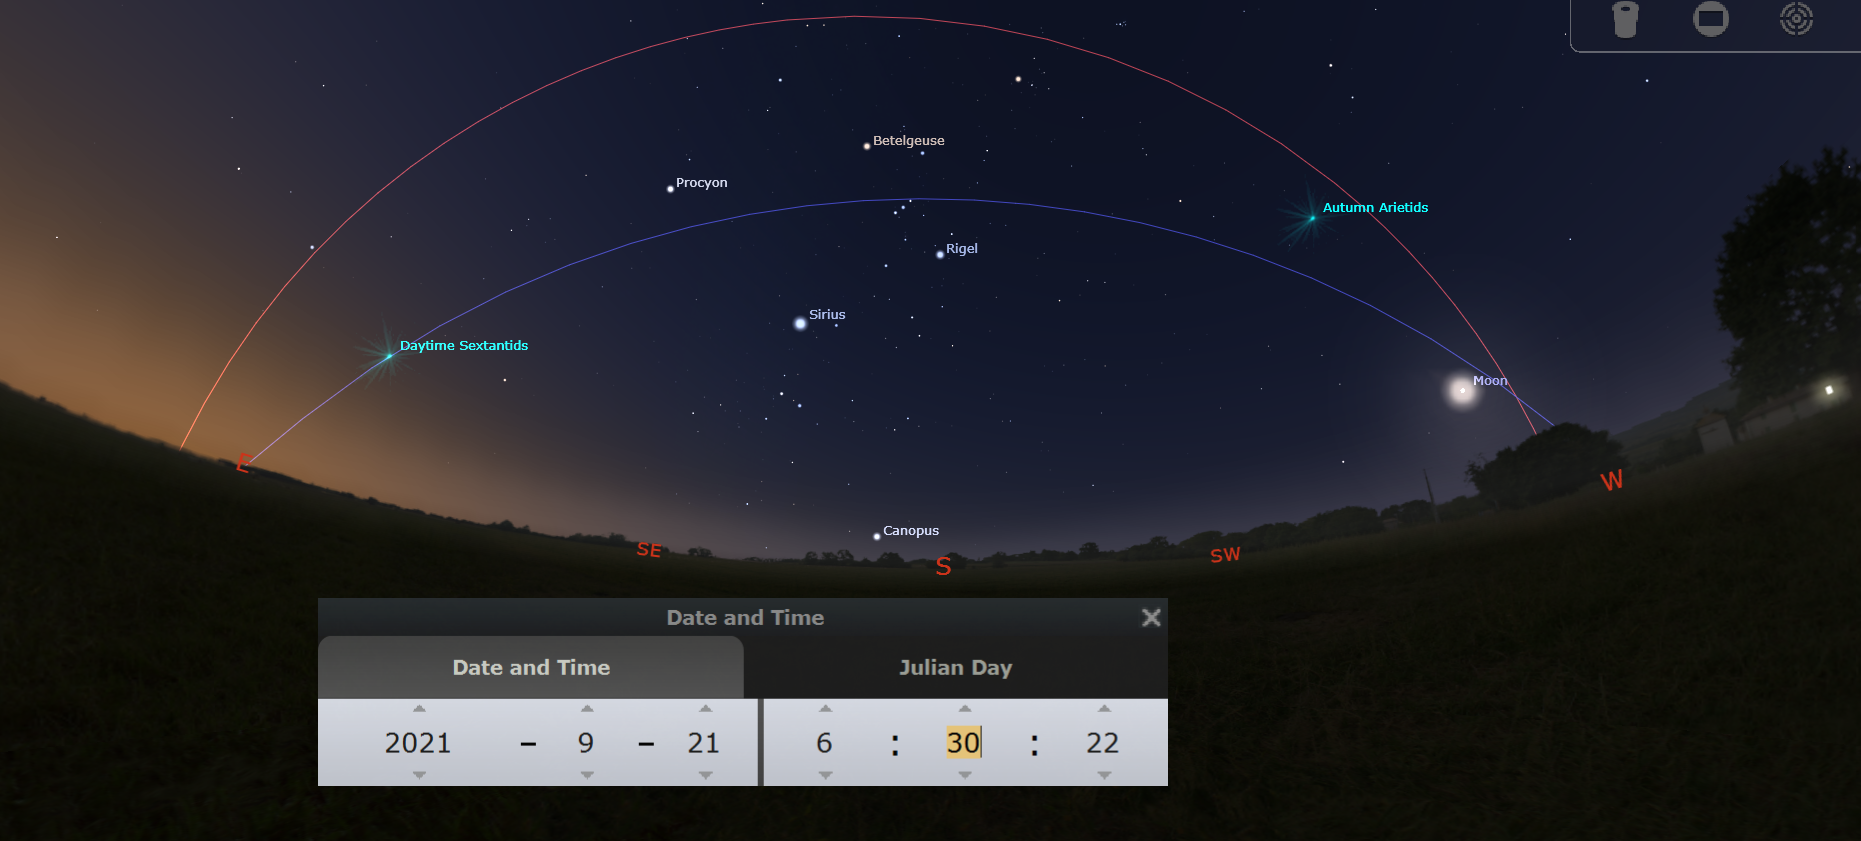
\includegraphics[width=4in]{Figures/Figure_Stellarium_Sunrise.png}
%     % \caption{Caption}
%     % \label{fig:my_label}
% \end{figure}

\textbf{Ecliptic}
\vspace{-1em}

\begin{enumerate}
\setlength\parskip{0pt}
    \item Open \textit{Stellarium}.
    \item Click \texttt[red]{Sky and viewing options window [F4]} and click the \texttt[red]{Markings} tab. Click the first \texttt[red]{Ecliptic~(J2000)} box and set the \texttt[red]{Thickness} of lines to 5. Close the window. 
    \item Face South and zoom out until the ecliptic path fills the frame. Click the  \texttt[red]{Date/time window [F5]} and advance time by 1-month intervals. What do you notice?
    \item Click \texttt[red]{Sky and viewing options window [F4]} and click the \texttt[red]{Starlore} tab. Under the \texttt{Options} section, check the boxes for \texttt[red]{Show labels}, \texttt[red]{Show constellation lines}, and \texttt[red]{Show art in brightness}. This allows you to see constellation lines and the art associated with their mythology. Close the window.
    \item Face South set the time to 12:00~PM. Click the  \texttt[red]{Date/time window [F5]} and advance time by 1-day intervals. What do you notice? Record your observations.
    \item Based on your observations, create a definition for \textbf{ecliptic}. 
    \item What is the textbook definition for \textbf{ecliptic}?
\end{enumerate}

\textbf{Ecliptic and Celestial Equator}
\vspace{-1em}

\begin{enumerate}
\setlength\parskip{0pt}
    \item Open \textit{Stellarium}.
    \item Set your location to Cypress, Texas.
    \item In the \texttt[red]{Sky and viewing options window [F4]} check the first \texttt[red]{Equator (J2000)} box and set \texttt[red]{Thickness} of lines to 5. Close the window.
    \item \label{lab:Stellarium_SetDate} Set the \texttt[red]{Date and time window [F5]} to June 21 at 12:00~PM.
    \item Face South and zoom in/out until the celestial equator fills your view.
    \item \label{lab:Stellarium_AdvanceTime} Set the time to 6:00~AM and advance it by 1 hour intervals until the Sun sets. Observe how the Sun moves across the sky and describe the proximity of the Sun to the celestial equator and to the horizon. Record your observations and draw a sketch.
    \item Repeat steps (\ref{lab:Stellarium_SetDate}) and (\ref{lab:Stellarium_AdvanceTime}) for the dates of September 21, December 21, and March 21. 
    \item What what is the significance of the 4 aforementioned dates? What can you conclude about the movement of the Sun across the sky on and between these dates?
    \item Re-do this whole exercise with the \textbf{ecliptic} included in the viewing options \texttt[red]{[F4]}. How does the ecliptic help you predict the position of the Sun relative to the celestial equator across the calendar year?
    
\end{enumerate}

\clearpage

\stepcounter{mycounter}

Astronomy \hfill Worksheet \themycounter \hfill Chapter 4
\vspace{1em}


\begin{enumerate}
\setlength\parskip{0pt}
    \item Open \textit{Stellarium}.
    \item Click \texttt[red]{Location window [F6]} and set location to \textit{Austin, Texas}. Close the window.
    \item Rotate the horizon so that you face southeast, with the Sun high in the sky.
    \item Click \texttt[red]{Date/time window [F5]}. Set the date to April 8, 2024 and the time to 12:45~PM. 
    \item Advance time by one minute intervals by clicking and holding the up arrow on the minute setting. Do this until the simulation time reaches 2:45~PM (14:45).
    \item Describe what happened across the 2 hour interval. Is there a name for this phenomenon?
\end{enumerate}


\end{document}